


\documentclass[12pt]{extarticle}

\usepackage{summary-intro}
%\usepackage{hyperref}

\newcommand{\ub}{\ensuremath{\underline{\enspace}}}
\usepackage{multicol}




\begin{document}
\sumintro{Computability}{Spring 2023}





\section{The Main Result}

\begin{itemize}

\item We'll focus on functions $f: \mathbb{N} \rightarrow \mathbb{N}$.

\item For a computer program to \textbf{compute} $f$ is for it to yield $f(n)$ as output whenever it is given $n$ as input ($n \in \mathbb{N}$). 

\item \emph{Theorem:} not every function is computable (we will see some examples).

%(And I can give you examples!)


\end{itemize}



\section{How We'll Get There}

\begin{itemize}

\item Turing Machines are computers of an especially simple sort.

\item We'll see that some functions are not Turing-computable.

\item But: any function that can be computed using an ordinary computer is also computed by some Turing Machine. 

\end{itemize}







\section{Turing Machines}




\subsection*{Hardware}

\begin{description}
\item[Memory tape] 
A long strip of paper (potentially infinite), divided into cells:

\begin{center}
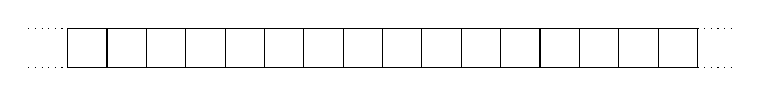
\begin{tikzpicture}
\draw (0,0) -- (8,0); % base horizontal
\draw[dotted] (8,0) -- (8.5,0); % base horizontal dots (right)
\draw[dotted] (-0.5,0) -- (0,0); % base horizontal dots (left)
\draw (0,0.5) -- (8,0.5); % top horizontal
\draw[dotted] (8,0.5) -- (8.5,0.5); % top horizontal dots (right)
\draw[dotted] (-0.5,0.5) -- (0,0.5); % top horizontal dots (left)


\draw (0,0) -- (0,0.5); % vertical
\draw (0.5,0) -- (0.5,0.5); % vertical
\draw (1,0) -- (1,0.5); % vertical
\draw (1.5,0) -- (1.5,0.5); % vertical
\draw (2,0) -- (2,0.5); % vertical
\draw (2.5,0) -- (2.5,0.5); % vertical
\draw (3,0) -- (3,0.5); % vertical
\draw (3.5,0) -- (3.5,0.5); % vertical
\draw (4,0) -- (4,0.5); % vertical
\draw (4.5,0) -- (4.5,0.5); % vertical
\draw (5,0) -- (5,0.5); % vertical
\draw (5.5,0) -- (5.5,0.5); % vertical
\draw (6,0) -- (6,0.5); % vertical
\draw (6.5,0) -- (6.5,0.5); % vertical
\draw (7,0) -- (7,0.5); % vertical
\draw (7.5,0) -- (7.5,0.5); % vertical
\draw (8,0) -- (8,0.5); % vertical


\end{tikzpicture}
\end{center}
(A unionized assistant is ready to add paper on either end, as needed.)

\item[Tape-reader]
At any given time, the reader is positioned on a cell of the memory tape and is able to perform any of the following functions: 

      \begin{itemize}
      \item Read the symbol written on the cell
      \item Write a new symbol on the cell
      \item Move one cell to the left
      \item Move one cell to the right
      \end{itemize}
\end{description}

\subsection*{Software}

A  finite list of \textbf{command lines}:
\[
\seq{\text{current state}} \seq{\text{current symbol}} \seq{\text{new symbol}} \seq{\text{direction}} \seq{\text{new state}}
\]
Think of a command line as encoding the following instruction:

\begin{quote}If you are in $\seq{\text{current state}}$ and your reader sees $\seq{\text{current symbol}}$ written on the memory tape, replace $\seq{\text{current symbol}}$ with $\seq{\text{new symbol}}$. Then move one step in direction $\seq{\text{direction}}$, and go to $\seq{\text{new state}}$.
\end{quote}

\subsection*{Operation}

\begin{itemize}

\item Begin in state 0. Then carry out the following procedure, for as long as you are able:

\begin{itemize}

\item Perform the instruction corresponding to the (first) command line that matches your current state and the symbol on which your reader is positioned.  


\item (Rinse \&) Repeat. 

\end{itemize}


\item If you are unable carry out the procedure, halt.


\end{itemize}

\section{A Turing Machine Simulator}

\url{http://morphett.info/turing/}



% in 2019 the lecture went great and ended here. We did a lovely exercise on the simulator in which we coded, moving to the right of a block of 0s and 1s, adding one in binary, subtracting one in binary, and finally using all of that to add two strings together. (It's important to make sure that the tally is on the right and the counter on the left, so that the tally has unlimited room to grow.) A demonstration is now captures as a MOOC video.


\section{Computing functions on a Turing Machine}

Computability:
\begin{itemize}

\item For a computer program to \textbf{compute} $f$ is for it to yield $f(n)$ as output whenever it is given $n$ as input. 

\end{itemize}

\noindent
Turing Computabiity:
\begin{itemize}

\item $M$ takes \(n\) ($n \in \mathbb{N}$) as \textbf{input} if it starts out with a tape that contains only a sequence of \(n\) ones (with the reader positioned at the left-most one, if $n > 0$).

\item  $M$ delivers \(f(n)\) as \textbf{output} if it halts with a tape that contains only a sequence of \(f(n)\) ones (with the reader positioned at the left-most one, if $n > 0$).

\item $M$ \textbf{computes} a function \(f(x)\) if and only if it delivers \(f(n)\) as output whenever it is given $n$ as input.

\end{itemize}






\section{The Main Result}

\begin{itemize}

\item We'll focus on functions $f: \mathbb{N} \rightarrow \mathbb{N}$.

\item For a computer program to \textbf{compute} $f$ is for it to yield $f(n)$ as output whenever it is given $n$ as input ($n \in \mathbb{N}$). 

\item \emph{Theorem:} not every function is computable.

%(And I can give you examples!)


\end{itemize}



\subsection{The Overall Plan}

\begin{itemize}

\item Turing Machines are computers of an especially simple sort.

\item We'll see that some functions are not Turing-computable.

\item But: any function that can be computed using an ordinary computer is also computed by some Turing Machine. 

\end{itemize}




\subsection{Computing functions on a Turing Machine}

\begin{itemize}

\item Simplifying Assumptions:
\begin{itemize}

\item We'll focus on \emph{one symbol} Turing Machines (where the only admissible symbols are ones and blanks).

\item We'll assume that the tape is only unbounded on the right.


\end{itemize}


\item Turing Computabiity:
\begin{itemize}

\item $M$ \textbf{computes} a function \(f(x)\) if and only if it delivers \(f(n)\) as output whenever it is given $n$ as input.


\item $M$ takes \(n\) ($n \in \mathbb{N}$) as \textbf{input} if it starts out with a tape that contains only a sequence of \(n\) ones (with the reader positioned at the left-most one, if $n > 0$).

\item  $M$ delivers \(f(n)\) as \textbf{output} if it halts with a tape that contains only a sequence of \(f(n)\) ones (with the reader positioned at the left-most one, if $n > 0$).


\end{itemize}
\end{itemize}











\subsection{Coding Turing Machines as Numbers}
\label{sec:numbering}

\subsubsection*{The Plan}


\[
\text{Turing Machine} \rightarrow \text{Sequence of symbols} \rightarrow
\text{Sequence of numbers} \rightarrow  \text{Unique number}
\]


\newpage

\subsubsection*{$\text{Sequence of symbols} \rightarrow \text{Sequence of numbers}$}


\begin{multicols}{3}



\begin{center}State Symbols:
\end{center}
\[
\begin{array}{ccc}
\text{``0''} &\rightarrow &\text{0}\\
\text{``1''} &\rightarrow &\text{1}\\
 &\vdots &
\end{array}
\]

\columnbreak

\begin{center}Tape Symbols:
\end{center}
\[
\begin{array}{ccc}
\text{``\ub''} &\rightarrow &\text{0}\\
\text{``$1$''} &\rightarrow &\text{1}\\
\
\end{array}
\]

\columnbreak

\begin{center}Movement Symbols:
\end{center}
\[
\begin{array}{ccc}
\text{``r''} &\rightarrow &\text{0}\\
\text{``$*$''} &\rightarrow &\text{1}\\
\text{``l''} &\rightarrow &\text{2}
\end{array}
\]



\end{multicols}


\subsubsection*{$ \text{Sequence of numbers} \rightarrow  \text{Unique number}$}

Codes the sequence  \(\seq{n_1, n_2, \ldots, n_k}\) as the number: \[p_{1}^{n_{1}+1}\cdot p_2^{n_2+1}\cdot\ldots\cdot p_k^{n_k+1}\] where \(p_i\) is the \(i\)th prime number.  

\vspace{5mm}
\noindent
(Treat any number that doesn't code a valid sequence of command lines as a code for the ``empty'' Turing Machine.) 




\subsection{An example}



$$2310 = 2\cdot 3\cdot 5\cdot 7\cdot 11$$
$$\downarrow$$
$$ 2^{0+1}\cdot 3^{0+1}\cdot 5^{0+1}\cdot 7^{0+1}\cdot 11^{0+1}$$
$$\downarrow$$
\[
\begin{array}{ccccc}
0 & 0 & 0 &0 &0\end{array}
\]
$$\downarrow$$
\[
\begin{array}{ccccc}
0 &\ub &\ub &r &0\end{array}
\]





\subsection{The Halting Function}


\begin{itemize}

\item $
H(n,m) =
\begin{cases}
1 \text{\quad if the \(n\)th Turning Machine halts when given input \(m\);}\\
0 \text{\quad otherwise.}
\end{cases}$
\vspace{1mm}

For instance: $H(2310, 0)=0$ and $H(2310, 2310)=1$.


\vspace{2mm}

\item$H(n) = H(n,n)$

\vspace{2mm}

For instance: $H(2310)=1$.
 
 \end{itemize}


\subsubsection{$\bm{H(n)}$ is not Turing-computable}




\begin{itemize}

\item Assume for \emph{reductio}: Turing Machine \(M^{H}\) computes \(H(n)\). 

\item Construct Turing Machine \(M^I\), which behaves as follows on input $k$:

\begin{description}
\item[Step 1:] Check whether $H(k)$ (using \(M^H\)). 

\item[Step 2:] 
$\begin{cases}
\text{If $H(k)=1$, go right forever.} \\

\text{If  $H(k)=0$, halt}.

\end{cases}$
\end{description}

\item \emph{Informally:} What happens when you run $M^I$ on input $\overline{M^I}$? It figures out whether it itself would halt on input $\overline{M^I}$. If the answer is yes, it goes off on an infinite task; if the answer is no, it immediately halts.

\item \emph{Formally:} $H(\overline{M^I})$ 1 or 0?

\begin{itemize}
\item Suppose $H(\overline{M^I}) = 1$. Then (by Step 2)  $M^I$ goes right forever on input $\overline{M^I}$. So $H(\overline{M^I}) = 0$.

\item Suppose $H(\overline{M^I}) = 0$. Then (by Step 2) $M^I$ halts on input $\overline{M^I}$. So $H(\overline{M^I}) = 1$.

\end{itemize}

\item So $M^I$ is impossible. So $M^H$ isn't computable after all.


\end{itemize}




\subsection{The Busy Beaver Function}


\begin{itemize}
\item $\bm{\text{\textbf{Productivity}}(M)} = \begin{cases} k,  \text{ if $M$ yields output $k$ on an empty input} \\ 0, \text{ otherwise}\end{cases}$

\item $\bm{BB(n)} = \ \mbox{\parbox{100mm}{the productivity of the most productive (one-symbol) Turing Machine with \(n\) states or fewer.}}$

\end{itemize}



\subsubsection{$\bm{BB(n)}$ is not Turing-computable}





\begin{itemize}

\item Assume for \emph{reductio}: Turing Machine \(M^{BB}\) computes \(BB(n)\). 

\item Construct Turing Machine \(M^I\), which behaves as follows on an empty input:

\begin{description}
\item[Step 1:]
Print a sequence of \(k\) ones, for a certain $k$ (specified below). 

\emph{Result:} $k$.

\item[Step 2:]
Duplicate your string of ones. 

 \emph{Result:} $2k$.

\item [Step 3]
Apply $BB$ to your string of ones (using \(M^{BB}\)).

 \emph{Result:} $BB(2k)$.

\item [Step 4]
Add one to your string of ones.

 \emph{Result:} $BB(2k)+1$.

\end{description}


\item Let $k =  b + c + d$

\begin{itemize}
\item[] \(b\) = the number of states used in Step 2 (to duplicate)

\item[] \(c\) = the number of states used in Step 3 (to apply $BB$)

\item[] \(d\) = the number of states used in Step 4 (to add one)

\end{itemize}
\emph{Note:} since a Turing Machine can output \(k\) using \(k\) states,

$$\overline{M^{I}} = k + b + c + d = 2k$$


\item $M^{BB}$ is impossible:

\begin{itemize}
\item At Stage~3, it produces as long a sequence of ones as a machine with $2k$ states could possibly produce. 

\item But (as noted above) $\overline{M^I} = 2k$. 

\item So at Stage~3, it produces as long a sequence of ones as it itself could possibly produce. 

\item So at Stage~4, it produces a \emph{longer} string of ones than it itself could possibly produce.

\end{itemize}



\item So $M^H$ isn't computable after all.


\end{itemize}




\section{The Universal Turing Machine}

There is a \textbf{Universal Turing Machine}, \(M^U\), which does the following:

\begin{itemize}
\item if the \(m\)th Turing Machine halts given input \(n\), leaving the tape in configuration \(p\), then
     \(M^U\) halts given input \(\seq{m,n}\) leaving the tape in configuration \(p\).
     
     \item if the \(m\)th Turing Machine never halts given input $n$, then \(M^U\) never halts given input \(\seq{m,n}\).
\end{itemize}


\clearpage

\section{The Fundamental Theorem}

The reason Turing Machines are so valuable is that it is possible to prove the following theorem:

\begin{description}
\item[Fundamental Theorem of Turing Machines]
A function from natural numbers to natural numbers is Turing-computable if and only if it can be computed by an ordinary computer, assuming unlimited memory and running time.

\end{description}


\begin{itemize}
\item  One shows that every Turing-computable function is computable by an ordinary computer (given unlimited memory and running time) by showing that one can program an ordinary computer to simulate any given Turing Machine.
\item  One shows that every function computable by an ordinary computer (given unlimited memory and running time) is Turing-computable by showing that one can find a Turing Machine that simulates any given ordinary computer.
\end{itemize}









\section{Church-Turing}
Computer scientists tend to think that something stronger than the Fundamental Theorem is true:

\begin{description}
\item[Church--Turing Thesis:] Every function that can be calculated by an effective method is Turing-computable.
\end{description}
(Note that the Church--Turing Thesis stated here may be different from the one stated in the MITx materials).

A method, $M$, for solving some problem is called \textbf{effective} just in case:


\begin{enumerate}%[label=(\roman*)]
\item $M$ is set out in terms of a finite number of exact instructions (each instruction being expressed by means of a finite number of symbols);
\item $M$ will, if carried out without error, produce the solution in a finite number of steps;
\item $M$ can (in practice or in principle) be carried out by a human being unaided by any machinery except paper and pencil (No special physical conditions are required for the computation to succeed---no need for faster-than-light travel, special solutions to Einstein's equations, etc)
\item $M$ demands no insight, intuition, or ingenuity, on the part of the agent carrying out the method.
\end{enumerate}


\iffalse %version of church--turing from earlier sheets, in MITx materials?

\begin{description}
\item[Church-Turing Thesis:]  A function is Turing-computable if and only if it can be computed algorithmically. 
\end{description}

For a problem to be solvable \textbf{algorithmically} is for it to be possible to specify a finite list of instructions for solving the problem such that:\label{gloss:algorithm}

\begin{enumerate}

\item Following the instructions is guaranteed to yield a solution to the problem, in a finite amount of time.

\item The instructions are specified in such a way that carrying them out requires no ingenuity of any kind: they can be followed mechanistically. 

\item No special resources are required to carry out the instructions: they could in principle be carried out by a machine built from transistors. %%this condition is plausibly better than the `pencil and paper' requirement above, which seems too restrictive! 

\item No special physical conditions are required for the computation to succeed (no need for faster-than-light travel, special solutions to Einstein's equations, etc).

\end{enumerate}

\fi 








\end{document}






